\documentclass{iagtese} 		% declara��o da classe iagtese com
						% padr�es de formata��o.
						%	
%\documentclass{iagtese_en}	% declara��o da classe iagtese em
						% ingles. Para escrever a tese em 
						% ingles, descomente esta linha e 
						% comente a linha anterior.
						%				%	
%\hypercolor				% links coloridos para a versao
						% on line da tese. Para usar esta
						% opcao descomente esta linha.
						% 	
\begin{document}			% in�cio do documento
						% 				
\institution{Universidade de S�o Paulo \\ Instituto de Astronomia, Geof�sica e Ci�ncias Atmosf�ricas \\ Departamento de Astronomia}

\title{T�tulo do trabalho}

\translator{{Tese/Disserta��o apresentada ao Departamento de Astronomia do Instituto de Astronomia, Geof�sica e Ci�ncias Atmosf�ricas da Universidade de S�o Paulo como requisito parcial para a obten��o do t�tulo de Mestre/{}Doutor em Ci�ncias.\\ \\
�rea de Concentra��o: Astronomia\\
Orientador(a): Prof.($^{\rm a}$) Dr.($^{\rm a}$) Orientador(a)}}

\author{Autor}

\date{S�o Paulo \ano}
			% arquivo para inserir a capa
						%
\pagestyle{empty}			% padr�o de formata��o para parte
						% inicial do texto
						%
\maketitle					% 
						%
\Dedicatoria				%
\hfill
\vfill
\hfill{\it{sua dedicatoria aqui!}}
\vspace{2cm}


		%
						% componentes iniciais do trabalho
\Agradecimentos			%
� minha fam�lia;

� fulana;

� orientadora;

Aos pesquisadores;

� Professora;

Aos colegas: 1, 2, 3 e 4

� FAPESP, pelo apoio financeiro, sob o projeto n$^o$: 6666/6666;

�s Institui��es

\vfill

\begin{flushleft}
\rule{6cm}{0.5pt}\\
{\footnotesize{Esta tese/disserta��o foi escrita em \LaTeX{} com a classe IAGTESE, para teses e disserta��es do IAG.}}
\end{flushleft}
	% caso n�o queira adicionar algum
						% deles, simplesmente remova as
						% linhas correspondentes.
						%
\Epigrafe					%  
\vfill
\begin{flushright}

``\textit{frase bonita 01}''\\

\vspace{0.4cm}

Autor da frase bonita 01

\end{flushright}

\vspace{0.5cm}

\begin{flushright}

``\textit{frase bonita 02}''\\

\vspace{0.4cm}

Autor da frase bonita 02

\end{flushright}

\vspace{2cm}
		%
						%
\Resumo					%

\resumo{Neste Relatório são apresentados os resultados do monitoramento sismológico efetuado na área da Usina Hidrelétrica Salto Pilão, por meio da Estação Sismológica SP7, no período entre 01.12.2022 e 30.06.2023, permitindo acompanhar a sismicidade local e orientar a adoção de eventuais medidas mitigadoras. Durante o monitoramento sismológico local efetuado, a Estação SP7 registrou sessenta e sete (67) desmontes em obras/pedreiras na região. No período de referência do presente relatório não foi observada a ocorrência de evento sísmico induzido pela implementação do Empreendimento da UHE Salto Pilão. Foram detectados 4 sismos naturais, sendo 3 destes sismos locais próximos à estação SP7, e um evento regional próximo à cidade de Iguape – SP, no estado de São Paulo em 2023-06-16 11:22:00 (UTC) com magnitude 4.0 mR. Ressalta-se a contribuição que este monitoramento sismológico está dando para a confirmação e a determinação dos parâmetros de eventos ocorridos no território brasileiro, em especial aqueles com epicentros nos estados de Santa Catarina e Rio Grande do Sul, e regiões vizinhas. Assim, recomenda-se que a Estação SP7 seja mantida em funcionamento, possibilitando dar continuidade ao melhor conhecimento da sismicidade local e regional, além do necessário acompanhamento da operação da Usina Hidrelétrica Salto Pilão.}{Sismologia; sismicidade; Salto Pilão; sismos induzidos; sismos naturais; detonações; UHE Salto Pilão.}

		%
						%
\Abstract					%
Abstract
		%
						%
\listoffigures 				% lista de figuras (opcional)
\listoftables 				% lista de tabelas (opcional)
\tableofcontents 			% sum�rio
						%
\cleardoublepage			%
\pagestyle{fancy}			% formata��o para corpo do texto
						%
\section{INTRODUÇÃO}
\par{Este Relatório integra o estudo sismológico em desenvolvimento pelo Consórcio Empresarial Salto Pilão - CESAP e o IPT, de acordo com a Proposta FIPT/IPT n° 59220/21 de 29 de junho de 2021 - “Monitoramento sismológico na área do AHE Salto Pilão, SC, entre julho/2021 e junho/2024”, em continuidade aos trabalhos iniciados em janeiro de 2007 (Carta Proposta CT-Obras/SG-233/06), referentes à implantação do programa de monitoramento da sismicidade induzida na Usina Hidrelétrica Salto Pilão - UHESP. O estudo visa o atendimento aos requisitos do Projeto Básico Ambiental - PBA deste empreendimento, em execução na bacia do rio Itajaí-Açu, nos municípios de Lontras, Ibirama e Apiúna, no Estado de Santa Catarina, dentro do Programa 3: Monitoramento dos Impactos Geológicos – Sub-Programa 3.2: Sismicidade Induzida, de acordo com a LAO – Licença Ambiental de Operação no 4.055/12 concedida pela Fundação do Meio Ambiente - FATMA do Estado de Santa Catarina, atualmente Instituto de Meio Ambiente de Santa Catarina - IMA.}

\subsection{Objetivo}
\par{O objetivo deste trabalho é apresentar os resultados do monitoramento sismológico efetuado na área da Usina Hidrelétrica Salto Pilão, com a Estação Sismológica SP7, entre 01 de dezembro de 2022 e 30 de junho de 2023, permitindo acompanhar a sismicidade local e orientar a adoção de eventuais medidas mitigadoras, atendendo às exigências previstas no processo de licenciamento ambiental do empreendimento.}
		%
\chapter{Base de dados}\label{database}

Base de dados. Citar figura \ref{identificador}.

\begin{figure}[!ht]
\begin{center}
\setcaptionmargin{1cm}
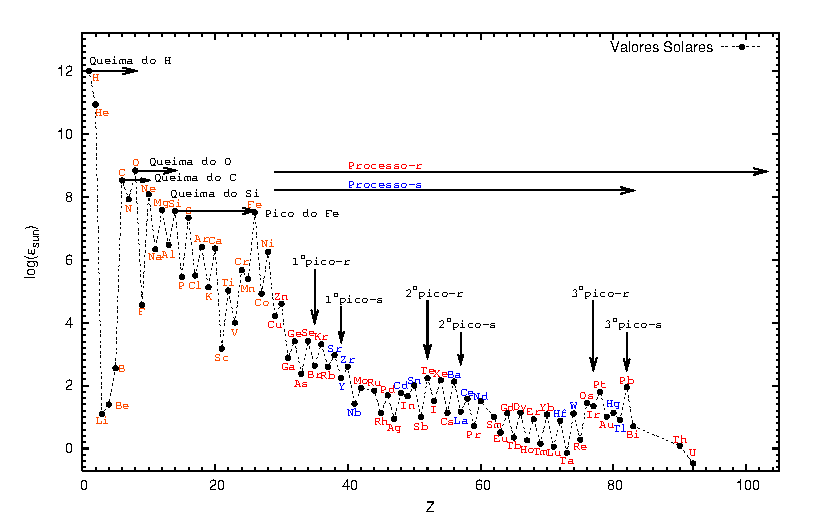
\includegraphics[width=1.0 \columnwidth,angle=0]{fig/solar_grevesse.eps}
\caption[Resumo da legenda da figura (aparece na lista de figuras)]{Legenda da figura.} 
\label{identificador}
\end{center}
\end{figure}


\begin{center}
\setcaptionmargin{1cm}
\scriptsize
\begin{longtable}{lcccc}
\caption[Resumo da legenda da tabela (aparece na lista de figuras)]{Exemplo de tabela feita com o longtable.}\\
\hline \hline \\[-2ex]
\multicolumn{1}{c}{Coluna1} &
\multicolumn{1}{c}{Coluna2} &
\multicolumn{1}{c}{Coluna3} &
\multicolumn{1}{c}{Coluna4} &
\multicolumn{1}{c}{Coluna5} 

\\[0.5ex] \hline
\\[-1.8ex]

\endfirsthead

\multicolumn{5}{c}{\footnotesize{{\slshape{{\tablename} \thetable{}}} - Continua��o}}\\[0.5ex]

\hline \hline\\[-2ex]

\multicolumn{1}{c}{Coluna1} &
\multicolumn{1}{c}{Coluna2} &
\multicolumn{1}{c}{Coluna3} &
\multicolumn{1}{c}{Coluna4} &
\multicolumn{1}{c}{Coluna5} 

\\[0.5ex] \hline
\\[-1.8ex]

\endhead

\multicolumn{3}{l}{{\footnotesize{Continua na pr�xima p�gina\ldots}}}\\
\endfoot
\hline

\endlastfoot

1 & 2 & 3 & 4 & 5 \\
6 & 7 & 8 & 9 & 10\\

\label{tabela_com_longtable}
\end{longtable}
\end{center}


    	% inserir os cap�tulos do seu
\chapter{An�lise}


An�lise
		% trabalho.
\chapter{Conclus�es}\label{conc}

Conclus�es do trabalho e/{}ou perspectivas
		% 
       						%
						%
%\begin{thebibliography}{99}	% refer�ncias bibliogr�ficas (d�
%\bibitem{Quireza et al. 2007}{quireza}Quireza C., Rocha-Pinto H. J., Maciel W. J., 2007, A\&A, 475, 217

\bibitem[Aoki et al.(2001)]{2001ApJ...561..346A} Aoki, W., Ryan, S. G., Norris, J. E., Beers, T. C., Ando, H., Iwamoto, N., Kajino, T., Mathews, G. J., \& Fujimoto, M. Y. 2001, ApJ 561, 346

\bibitem[Aoki et al.(2002)]{2002ApJ...580.1149A} Aoki, W., Ryan, S. G., Norris, J. E., Beers, T. C., Ando, H., \& Tsangarides, S. 2002, ApJ 580, 1149 

\bibitem[Wasserburg et al. (1994)]{1994ApJ...424..412W} Wasserburg, G. J., Busso, M., Gallino, R., \& Raiteri, C. M. 1994, ApJ 424, 412
 	% prefer�ncia ao bibTeX).
%\end{thebibliography}		% caso n�o use o bibTeX, remova os
						% comentarios das tr�s linhas
						% e comente a linha \bibliography
						%
\bibliography{tex/bibliografia}	% bibliografia utilizando bibTeX,
						% referente ao arquivo
						% bibliografia.bib na pasta tex/
						%
\begin{apendice}			% inicio do ambiente apendice
\chapter{t�tulo do ap�ndice 01}\label{ap01}

\section{subt�tulo 01}\label{subap01}

\chapter{t�tulo do ap�ndice 02}\label{ap02}
		% texto referente ao apendice
\end{apendice}				% fim do ambiente apendice. caso
						% nao utilize apendice, remova as
						% 3 linhas de comando.
						%
\end{document}				% fim do arquivo
